%!TEX program = xelatex
% 完整编译: xelatex -> bibtex -> xelatex -> xelatex
\documentclass[lang=cn,11pt,a4paper,cite=super,AutoFakeBold]{elegantpaper}

\title{基于Framingham数据集冠心病生存分析}
\author{蒋文馨 \quad 16342067 \quad
   \email{jiangwx7@mail2.sysu.edu.cn}}
\institute{中山大学数学学院17级统计学}
\date{\zhtoday}

% 本文档命令
\usepackage{array}
\usepackage{caption}
\usepackage{subcaption}
\newcommand{\ccr}[1]{\makecell{{\color{#1}\rule{1cm}{1cm}}}}

\begin{document}
\maketitle
\thispagestyle{empty}
\begin{abstract}
   \textbf{目的}\quad 探究导致冠心病(CHD)发病的高风险因素,建立可以用于预测
   CHD发病率的模型。\textbf{方法}\quad
   基于Framingham 心脏研究数据集,选择1956年马萨诸塞州Framingham社区
   无 CHD 病史的4,240名参与者纳入研究。探索分析
   临床数据的分布情况,使用多重填补法补全缺失值。
   采用Cox比例风险模型、AFT模型和考虑竞争风险的随机生存森林模型进行统计分析,
   利用列线图实现在给定条件下的 CHD 患病概率的预测。
   \textbf{结果}\quad 1,046名参与者在24年的随访期内发展为CHD。
   多因素Cox比例风险模型认为,糖尿病(Hazard Ratio,HR  = 2.2,95\%CI:1.7$ \sim$ 2.9 ),
   性别(男性)(HR  = 2.1 ,95\%CI:1.9 $\sim$2.4 ),
   中风病史(HR  = 1.6,95\%CI:0.9 $\sim$3.1 ),
   服用降压药(患有高血压)(HR  = 1.3,95\%CI:1.0 $\sim$1.7 ),
   吸烟(HR  = 1.2,95\%CI:1.1 $\sim$1.4 )等是CHD发生的危险因素。
   \textbf{结论}\quad 性别(男性)、高龄、血清总胆固醇增高、肥胖、
   吸烟、患糖尿病、有中风史、高血压是CHD的危险因素,对预测患病率有极大帮助。
   \keywords{Framingham心脏研究 \quad 冠心病 \quad 生存分析 \quad Cox模型 \quad 
    竞争风险随机生存森林 }

\end{abstract}
%\newpage
%\setcounter{page}{1}
\setcounter{tocdepth}{1}
\tableofcontents
\thispagestyle{empty}
\newpage

\setcounter{page}{1}
\setcounter{section}{-1}
\section{引言}
冠心病(Coronary Heart Disease,CHD)是全球主要的死亡原因~\cite{firstblood}。
当向心肌输送氧气的冠状动脉由于脂肪或胆固醇在动脉壁内堆积而变窄或被阻塞时,就会发生冠心病。
高风险因素包括:高胆固醇(总胆固醇过高或低密度脂蛋白胆固醇过高、高密度脂蛋白胆固醇过低)、
抽烟、高血压、糖尿病、缺乏运动、肥胖、不良的饮食习惯、高龄、心脏病家族史、
心脏病既往病史等~\cite{2blood}~\cite{3blood}。

为进一步探索导致CHD的因素,本文使用 Framingham 心脏病数据集,完成以下四个任务:
\begin{itemize}
   \item 建立CHD生存分析模型;
   \item 探究高风险因素对CHD发病率的影响;
   \item 探究竞争风险对CHD发病率的影响;
   \item 预测在给定条件下的CHD患病概率。
\end{itemize}


\section{数据说明}
Framingham心脏研究是一项针对马萨诸塞州Framingham社区中自由生活的人群中心血管疾病病因的长期前瞻性研究,
已成为全球心血管健康最重要的研究之一。这项研究明确了导致各类心血管疾病的高危因素,从而得出针对这些疾病的有效治疗方法~\cite{70y}。
本文所用数据集是Framingham研究的一部分数据的一部分,包括4,434名参与者的实验室、诊所、调查表和裁决事件数据。
在大约1956年至1968年的三个检查阶段中(大约相隔6年)收集了参与者的临床数据。每个参与者的随访时间总计为24年,
其结果为以下事件:心绞痛、心肌梗塞、动脉血栓形成梗塞或脑出血(中风)或死亡。 
数据以纵向形式提供。根据参加者的检查次数,每个参与者有1到3个观察结果,因此,对4,434名参与者有11,627个观察结果。
\begin{table}[htb]
   \centering
   \caption{研究对象基线情况(n = 4434)}
   \label{tab:sjsm}
   \resizebox{\textwidth}{!}{
   \begin{tabular}{lll||lll} 
   \toprule
   列名       & 项目             & 取值            & 列名        & 项目              & 取值        \\
   \midrule
   randid   & 编号             & -             & \multicolumn{2}{l}{第一次检查数据} &           \\
   疾病       &  & & totchol1  & 血清总胆固醇(mg/dL)   & 234(206,264)[52]        \\
   death    & 死亡[例(\%)]      & 1550(33.16\%) & age1      & 年龄              & 49(42,57) \\
   anychd   & 冠心病[例(\%)]     & 1240(24.67\%) & sysbp1    & 收缩压(mmHg)       & 129(117.5,144)          \\
   hyperten & 高血压[例(\%)]     & 3252(73.34\%) & diabp1    & 舒张压(mmHg)       & 82(75,90) \\
   时间       &  & & cursmoke1 & 吸烟[例(\%)]       & 2181(49.19\%)           \\
   timedth  & 死亡时间           & 0-24          & cigpday1  & 每日吸烟数量          & 0(0,20)[32]             \\
   timechd  & 患冠心病时间         & 0-24          & bmi1      & 体重指数            & 25.45(23.09,28.09)[19]  \\
   timehyp  & 患高血压时间         & 0-24          & diabetes1 & 糖尿病[例(\%)]      & 121(2.73\%)             \\
   性别       &  & & bpmeds1   & 使用降压药[例(\%)]    & 144(3.25\%)[61]         \\
   Female   & 男性[例(\%)]      & 1944(43.84\%) & heartrte1 & 心率(beats/min)   & 75(68,83)[1]            \\
   Male     & 女性[例(\%)]      & 2490(56.16\%) & glucose1  & 血糖(mg/dL)~      & 78(72,87)[397]          \\
   病史       &  & &           &   &           \\
   prevchd1 & 冠心病既往病史[例(\%)] & 194(4.38\%)   &           &   &           \\
   prevstrk1& 中风既往病史[例(\%)] & 32(7.22\%)   &           &   &           \\
   prevhyp1 & 高血压既往病史[例(\%)] & 1430(32.25\%) &           &   &           \\
   \bottomrule
   \multicolumn{6}{r}{\small{[*]表示缺失数目}}\\
   \end{tabular}}
\end{table}

本文涉及项目的人群的基线情况及数据的说明见表\ref{tab:sjsm}。因大多数连续型变量均为
非正态分布,故数据(除时间以外)表示为中位数(下四分位数,上四分位数);[*]表示缺失数目;
生存时间为0表示在检查开始前就有病史,为24表示右删失。第二次和
第三次检查的数据与第一次形式类似,故省略。可以看出数据集中有多个缺失值,我们假设数据为
随机缺失 (missing at random,MAR),即数据的缺失不是完全随机的,该类数据的缺失依
赖于其他完全变量。对于第二次和第三次检查,一些参与者因为死亡(竞争风险)等原因退出实验导致右删失,
或者缺席某次检查,这也导致数据缺失。

\section{探索性分析和预处理}
多因素Cox比例风险模型仅使用不含有缺失值的信息,缺失值的大量出现将导致信息的丢失。因此对于
本数据集而言,缺失值填补十分必要。接下来,将以第一次检查的数据为例,探究缺失值的分布情况,寻找
合适的填补方案,再对三次检查的数据进行填补。由于数据集项目大多为连续型变量,需要对极端值进行处理。
最后选取无 CHD 病史的参与者纳入后续分析研究并讨论数据右删失情况。
\subsection{缺失值处理}
数据集中缺失值主要有两种情况。一是单一缺失值,即缺失值单独出现;二是整次检查数据缺失,
即缺席第二或第三次检查。对于仅缺失第二次检查的57名参与者,使用第一次和第三次检查的平均值代替缺失值。
对于单一缺失值,利用第一次测试的数据,探索项目的分布及项目之间的关系。单一缺失值主要出现在血糖、
使用降压药、血清总胆固醇和每日吸烟数量。
日均吸烟量缺失的参与者全部都在吸烟,而对于吸烟的参与者,其日均吸烟量分布直方图如图\ref{fig:rjxyzft}所示。
为补全血糖的缺失值,探究糖尿病患者和非患者的血糖分布情况如图\ref{fig:tnbxt}所示,可以看出
糖尿病患者与非患者血糖分布情况有很大的差异。为补全是否使用降压药这一项,探究是否使用降压药和舒张压收缩压之间的关系,
如图\ref{fig:ssyjyy}和\ref{fig:szyjyy}所示,虽然缺失值的分布近似于没有使用降压药的分布,但由于绝大多数参与者
都未使用降压药,所以对于该缺失值仍需进一步讨论才可填充。

   \begin{figure}[!hbt]
      \begin{subfigure}[b]{0.49\textwidth}
        \centering
        % include 1 image
        \includegraphics[width=0.8\linewidth]{img/cig1-1.pdf}  
      \caption{日均吸烟数分布直方图}
      \label{fig:rjxyzft}
      \end{subfigure}
      \begin{subfigure}[b]{0.49\textwidth}
        \centering
        % include 2 image
        \includegraphics[width=\linewidth]{img/glu2-1.pdf}  
        \caption{糖尿病患者与非患者血糖分布核密度图}
        \label{fig:tnbxt}
      \end{subfigure}
      ~
      \begin{subfigure}[b]{0.49\textwidth}
         \centering
         % include 3 image
         \includegraphics[width=\linewidth]{img/sys3-1.pdf}  
       \caption{收缩压与是否服用降压药分布核密度图}
       \label{fig:ssyjyy}
       \end{subfigure}
       \begin{subfigure}[b]{0.49\textwidth}
         \centering
         % include 4 image
         \includegraphics[width=\linewidth]{img/dia4-1.pdf}  
         \caption{舒张压与是否服用降压药分布核密度图}
         \label{fig:szyjyy}
       \end{subfigure}
      \caption{探索项目间关系}
   \end{figure}

根据数据集的特点,选取如下3种填补方法:
\begin{enumerate}
   \item 中位数填补:使用该项目的中位数填补缺失值;
   \item 随机森林:使用randomForestSRC包的impute()生成随机森林模型预测缺失值;
   \item 多重填补(Multivariate Imputation,MI):
   一种基于重复模拟的处理缺失值方法,处理复杂的缺失值问题最常选用的方法。
   这里采用mice包利用链式方程的多元插补(Multivariate Imputation via Chained Equations,MICE)完成。
   mice()中,缺失值的插补通过Gibbs抽样完成。每个包含缺失值的变量都默认可通过数据集中的其他变量预测得来, 
   于是这些预测方程便可用来预测缺失数据的有效值 ~\cite{ria}。mice()填补过程示意图如图\ref{fig:mice}所示。
   \begin{figure}[!htbp]
      \centering
      \includegraphics[width=0.7\linewidth]{img/mice.jpg}
      \caption{通过MICE包应用多重插补的步骤:函数mice()首先从一个包含缺失数据的数据框开始,然后
      返回一个包含多个(默认为5个) 完整数据集的对象。 每个完整数据集都是通过对原
      始数据框中的缺失数据进行插补而生成的。 由于插补有随机的成分,因此每个完整数
      据集都略有不同。然后,with()函数可依次对每个完整数据集应用统计模型(如线性模
      型或广义线性模型) 。最后,pool()函数将这些单独的分析结果整合为一组结果。最终模
      型的标准误和p值都将准确地反映出由于缺失值和多重插补而产生的不确定性。}
      \label{fig:mice}
   \end{figure}
\end{enumerate}

为测试不同填补方式的效果,先在第一次检查的数据中进行填补。通过对比不同填补方式填补后数据的分布(例如平均数,
中位数,上下四分位数等),
结合上文对于数据分布的分析,同时根据参考文献~\cite{mi}的建议,最终选取的方法为多重填补。

确定填补方法后,考虑到三次检查进行时间间隔较久,且有数据删失,故对三次检查分开填补。至此,缺失值处理完毕。

\subsection{多重共线性问题}
舒张压和收缩压有极大的相关性,这会影响回归系数的稳定性,一般计算平均动脉压(Mean Arterial Pressure,MAP),
定义为舒张压和收缩压的加权平均~\cite{helpstar}:
$$MAP=\frac{SBP + 2\times DBP}{3}.$$

\subsection{极端值处理}
在开始任何建模之前,应仔细检查所有潜在预测变量的分布以获取极值。 
最好将数据与原始文档进行核对,但有时必须根据常识做出此类决策。 
可以将生物学上难以置信的值设置为缺失值,并通过将值从1个百分点以下和99个
百分点以上移至“截断点”来截断剩余的极端值。 
这种截断可以防止由于极值的高杠杆作用而导致预测变量和结果之间的关系失真~\cite{helpstar}。

通过对数据集每个变量绘制箱型图判断极端值情况,可知存在较多极端值的项目为日均吸烟数
(如图\ref{fig:rjxyzft}所示)和心率(如图\ref{fig:hrtrate}所示)。
由于人类心率受状态(运动,休息)的影响大于是否患有心脏病,故应多时间点测量取平均心率。
考虑到数据集的特点,这里定义下文参与者的心率为个体参与多次(实际参与次数)检查的平均心率。
\begin{figure}[htb]
   \centering
   \includegraphics[width=0.6\linewidth]{img/pal-1.pdf}
   \caption{三次检查心率变化图}
   \label{fig:hrtrate}
\end{figure}

\subsection{选择无CHD病史的参与者}
因为本文分析方向为高危因素对CHD发病的影响,故应选择无CHD病史(即第一次检查时
无CHD病史)的4240名参与者纳入研究。
此后的分析均基于这4240位参与者。

\subsection{删失}
从图\ref{fig:survc}可以看出,存在大量右删失数据。分析数据可知,824个右删失是由竞争风险(比如死亡)
导致的,2341个右删失是因为研究结束后CHD仍未发生。这里假设删失是独立的,
且患CHD与删失无关(non-informative)。
\begin{figure}[htb]
   \centering
   \includegraphics[width=0.6\linewidth]{img/survc.pdf}
   \caption{KM曲线图}
   \label{fig:survc}
\end{figure}

\section{数据分析}
这一部分将使用Cox比例风险模型、扩展的分层Cox比例风险模型、
基于三次检查的扩展Cox比例风险模型、AFT模型和竞争的随机生成森林模型进行建模分析。
使用C-index度量模型的性能。
为了方便建模、减少运算量,首先仅使用第一次检查的数据,待建立完模型后,使用扩展的Cox
模型,引入后两次检查的数据\footnote{由于电脑算力有限,尽量建立简单的模型}。
\subsection{Cox比例风险模型}
\subsubsection{单因素Cox比例风险模型}
\begin{table}[htb]
   \centering
   \caption{单因素Cox比例风险模型}
   \label{tab:unicoxph}
   %  \resizebox{\textwidth}{!}{
      \setlength{\tabcolsep}{7mm}{
\begin{tabular}{cccccc} 
   \toprule
   项目       & Wald test & df & p值     & HR    & 95\%CI           \\
   \midrule
   sex       & 107.8       & 1  & <2e-16  & 1.910 & 1.691-2.158      \\
   totchol1  & 134.8       & 1  & <2e-16  & 1.007 & 1.005-1.008      \\
   age1      & 175.1       & 1  & <2e-16  & 1.049 & 1.042-1.057      \\
   sysbp1    & 260         & 1  & <2e-16  & 1.020 & 1.017-1.022      \\
   diabp1    & 164.7       & 1  & <2e-16  & 1.031 & 1.027-1.036      \\
   cursmoke1 & 1.4         & 1  & 0.236  & 1.076 & 0.953-1.215      \\
   cigpday1  & 12.38       & 1  & 4e-3   & 1.009 & 1.004-1.014      \\
   bmi1      & 107.1       & 1  & <2e-16  & 1.072 & 1.058-1.086      \\
   diabetes1 & 74.48       & 1  & <2e-16  & 3.316 & 2.525-4.353      \\
   bpmeds1   & 40.19       & 1  & <2e-16  & 2.447 & 1.856-3.227      \\
   heartrte1 & 0.25        & 1  & 0.615  & 0.999 & 0.994-1.004      \\
   heartrte  & 1.16        & 1  & 0.281  & 1.003 & 0.997-1.009      \\
   glucose1  & 69.46       & 1  & <2e-16  & 1.008 & 1.006-1.010      \\
   map1      & 232.6       & 1  & <2e-16  & 1.030 & 1.026-1.033      \\
   prevstrk1 & 6.33        & 1  & 0.012  & 2.323 & 1.205-4.478      \\
   prevhyp1  & 146.2       & 1  & <2e-16  & 2.133 & 1.887-2.412      \\
   \bottomrule
   \multicolumn{6}{l}{MAX C-index(se) = 0.59 ( 0.008 ) }\\
\end{tabular}}
\end{table}

首先对每个项目建立单因素Cox比例风险模型,以初步判断单个项目对CHD生存情况的影响。
结果如表\ref{tab:unicoxph}所示。其中heartrte1表示第一次检查的心率,heartrte
表示多次检查的平均心率。一般而言,心率越高,越有可能患CHD~\cite{2blood}。
然而heartrte1的HR小于1,与之矛盾。heartrte的HR大于1,且p值比heartrte1的p值
更小。故使用heartrte进行建模更为合适。此外,可知性别、患有糖尿病、中风史、高血压史和使用降压药
的参与者有更高的风险患CHD。虽然降压药不一定导致CHD,但是使用降压药预示着参与者
血压过高,这会增加患CHD的几率。

由于仅有当前是否吸烟和心率p值大于0.20,故待后续分析后再进行变量筛选。

\subsubsection{多因素Cox比例风险模型}
对表\ref{tab:unicoxph}中除heartrte1和diabp1(和sysbp1有共线性)外所有变量建立多因素
Cox比例风险模型,结果如表\ref{tab:multicoxph}所示。其中,最后一列为拟合优度检验的p值,
该值低于0.05表示变量不符合PH假设。该模型的C-index为0.71。

\begin{table}[htb]
   \centering
   \caption{多因素全变量Cox比例风险模型}
   \label{tab:multicoxph}
   \setlength{\tabcolsep}{5mm}{
   \begin{tabular}{ccccccc}
   \toprule
             & coef       & exp(coef)       & se(coef)       & z       & p   & \text{拟合优度}-p\\
   \midrule
   sex       & 0.722      & 2.058           & 0.069          & 10.53   & <2e-16   &0.34  \\
   totchol1  & 0.005      & 1.005           & 0.001          & 7.80    & 6.15e-15         &0.02  \\
   age1      & 0.034      & 1.035           & 0.004          & 8.12    & 4.77e-16         & <0.01 \\
   map1      & 0.000      & 1.000           & 0.006          & 0.01    & 0.9902         &  0.06\\
   cursmoke1 & 0.104      & 1.110           & 0.098          & 1.06    & 0.2887         &  0.28\\
   cigpday1  & 0.007      & 1.007           & 0.004          & 1.71    & 0.0866         &  0.01\\
   bmi1      & 0.035      & 1.036           & 0.008          & 4.41    & 1.02e-05         &  0.15\\
   diabetes1 & 0.529      & 1.697           & 0.188          & 2.81    & 0.0050         &  0.59\\
   sysbp1    & 0.012      & 1.013           & 0.004          & 2.96    & 0.0031         & 0.05 \\
   bpmeds1   & 0.265      & 1.303           & 0.152          & 1.74    & 0.0812         &  0.42\\
   heartrte  & -0.003     & 0.997           & 0.003          & -1.09   & 0.2775         &  0.54\\
   glucose1  & 0.003      & 1.003           & 0.001          & 2.47    & 0.0135         &  0.41\\
   prevstrk1 & 0.436      & 1.547           & 0.342          & 1.28    & 0.2024         &  0.29\\
   prevhyp1  & 0.049      & 1.050           & 0.089          & 0.55    & 0.5810       &   0.01\\
   \bottomrule
   \multicolumn{7}{l}{Likelihood ratio test = 560.5  on 14 df, p =< 2.2e-16}\\
   \multicolumn{7}{l}{n = 4240, number of events = 1046}\\
   \multicolumn{7}{l}{C-index(se) = 0.71(0.008 ) }\\
\end{tabular}}
\end{table}

从拟合优度检验的p值可以看出age1、totchol1、prevhyp1和cigpday1不符合PH假设。
考虑使用分层的Cox模型或扩展的Cox模型,以使模型符合PH假设。

接下来,以age1、heartrte、totchol1、prevhyp1和cigpday1为例,对变量进行分析。
\begin{itemize}
   \item \label{item:age} 年龄:\\
   对于年龄,常见的处理方式是分层,即认为40岁以下为低风险,40岁以上为高风险。然而数据集中40岁以下人数较少,
   第一次检查时为556人,第二次检查时为7人。故考虑将年龄划分为:(0,40),[40,50),[50,60),[60,81] 。
   KM曲线如图\ref{fig:km1}所示,可以看出几个年龄段生存曲线有明显不同,年龄越大生存函数下降越快,对数秩检验p值小于0.0001。
   从几条KM曲线间距趋势来看,这里可以考虑采用分层的Cox模型。
   
   \item 心率:\\一般认为心率超过100,会增加患CHD的风险~\cite{2blood}。故将三次检查的
   平均心率划分为小于100和大于等于100两类,绘制KM曲线,如图\ref{fig:km2}所示。虽然两类人群的生存函数
   有显著差异,对数秩检验p值为0.012。但该数据集心率大于等于100的人数较少,且心率有一定的误差(取了三次检查的平均),
   故对该数据集而言,心率不是一个很好的预测指标。

   \item 血清总胆固醇:\\高胆固醇(总胆固醇过高或低密度脂蛋白胆固醇过高、高密度脂蛋白胆固醇过低)
   为CHD高风险因素~\cite{3blood}。医学上认为总胆固醇高于200mg/dL 就会增加患心血管疾病的风险~\cite{chol}。

   \item 日均吸烟量:\\日均吸烟量相对于是否吸烟,能带来更多的信息量。因为不吸烟的参与者日均
   吸烟量为0。绘制KM曲线\ref{fig:km4}后发现少量吸烟的参与者患CHD几率小于不吸烟的参与者,且两条
   KM曲线没有交叉。我认为这是研究队列带来的偏差。

   \item 高血压病史:\\患有高血压会显著增加患CHD的风险~\cite{2blood},如图\ref{fig:km5}所示,对数秩检验p值小于0.0001。
\end{itemize}
\begin{figure}[!htbp]
   \begin{subfigure}[b]{0.49\textwidth}
     \centering
     % include 1 image
     \includegraphics[width=\linewidth]{img/km-1.pdf}  
   \caption{年龄KM曲线}
   \label{fig:km1}
   \end{subfigure}
   \begin{subfigure}[b]{0.49\textwidth}
     \centering
     % include 2 image
     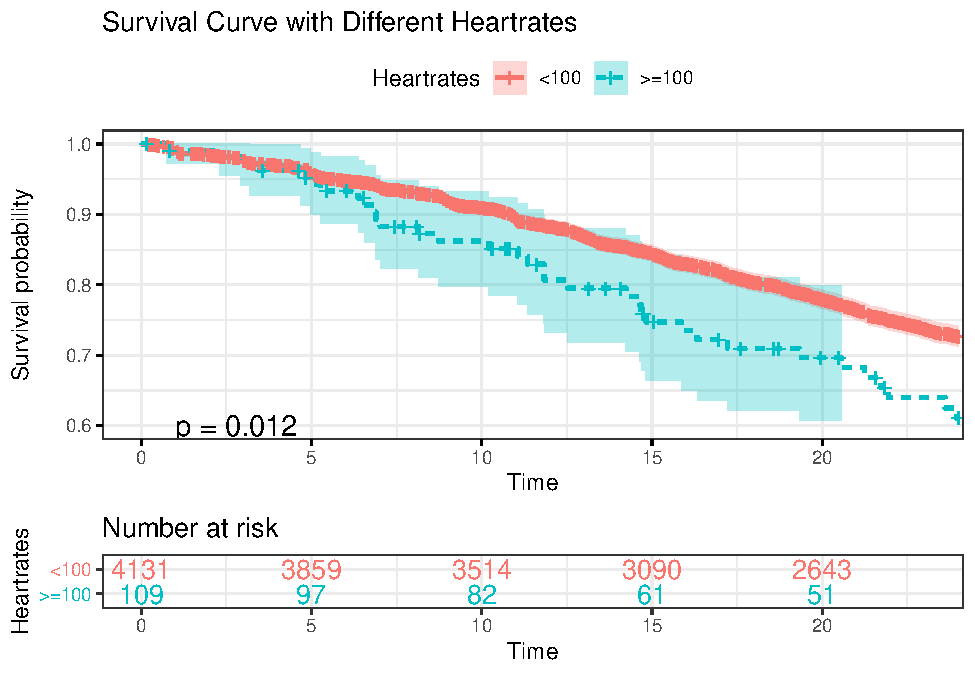
\includegraphics[width=\linewidth]{img/km-2.pdf}  
     \caption{心率KM曲线}
     \label{fig:km2}
   \end{subfigure}
   ~
   \begin{subfigure}[b]{0.49\textwidth}
      \centering
      % include 3 image
      \includegraphics[width=\linewidth]{img/km-3.pdf}  
    \caption{血清总胆固醇KM曲线}
    \label{fig:km3}
    \end{subfigure}
   \begin{subfigure}[b]{0.49\textwidth}
      \centering
      % include 3 image
      \includegraphics[width=\linewidth]{img/km-4.pdf}  
    \caption{日均吸烟量KM曲线}
    \label{fig:km4}
    \end{subfigure}
    ~
    \begin{center}
    \begin{subfigure}[t]{0.49\textwidth}
      \centering
      % include 5 image
      \includegraphics[width=\linewidth]{img/km-5.pdf}  
      \caption{高血压病史KM曲线}
      \label{fig:km5}
    \end{subfigure}       
    \end{center}
   \caption{KM曲线}
\end{figure}


根据上述分析,根据回归系数p值大小选择变量建立Cox比例风险模型和分层Cox比例风险模型。同时使得模型尽可能简单、
有较高的C-index且拟合优度检验满足PH假设。最终建立模型如表\ref{tab:mulcoxph}所示,该模型的C-index为0.71。
和使用全部变量的Cox模型相同。但此模型使用了更少的变量,故优于全变量 Cox模型。
左侧为不含分层的标准Cox比例风险模型,HR森林图如图\ref{fig:mulcox1}所示。可以看出变量系数显著,其中,
性别为男性、患有糖尿病为显著的高风险因素;而吸烟等其余因素均会导致CHD。
由拟合优度检验p值知,年龄不满足PH假设,故对年龄进行分层,如上述分析第\ref{item:age}点所述。

右侧为分层后的Cox比例风险模型,该模型的C-index为0.69,
Schoenfeld残差图如图\ref{fig:mulcox2}所示,总体而言模型符合PH假设\footnote{这里尝试过建立带交叉项的模型,但效果不好。}。
因Beta(t)随时间推移有下降的趋势,猜测bmi和cursmoke1为时依协变量,故接着建立扩展的Cox模型。

\begin{table}[hbt]
   \centering
   \caption{多因素Cox比例风险模型}
   \label{tab:mulcoxph}
   % \resizebox{\textwidth}{!}{
    \setlength{\tabcolsep}{4mm}{
   \begin{tabular}{ccccc||cccc} 
   \toprule
    & \multicolumn{4}{c}{标准的Cox模型}      & \multicolumn{4}{c}{分层的Cox模型}\\
   \midrule
             & HR    & p     & chisq  & p     & HR    & p     & chisq  & p      \\
   \midrule
   sex       & 2.140 & <2e-16 & 0.954  & 0.329 & 2.124 & <2e-16 & 2.630  & 0.105  \\
   age1      & 1.035 & <2e-16 & 13.875 & <e-3   & -     & -     & -      & -      \\
   totchol1  & 1.005 & <e-3   & 5.436  & 0.020 & 1.005 & <e-3   & 1.497  & 0.221  \\
   bmi1      & 1.036 & <e-3   & 1.881  & 0.170 & 1.036 & <e-3   & 1.283  & 0.257  \\
   cursmoke1 & 1.235 & 0.001 & 1.150  & 0.284 & 1.225 & 0.002 & 4.112  & 0.043  \\
   diabetes1 & 2.193 & <e-3   & 0.128  & 0.720 & 2.131 & <e-3   & 0.431  & 0.512  \\
   prevstrk1 & 1.589 & 0.176 & 1.074  & 0.300 & 1.561 & 0.194 & 0.410  & 0.522  \\
   sysbp1    & 1.013 & <2e-16 & 3.833  & 0.050 & 1.013 & <2e-16 & 0.330  & 0.565  \\
   bpmeds1   & 1.291 & 0.091 & 0.643  & 0.423 & 1.317 & 0.068 & 0.055  & 0.815  \\
   GLOBAL    & -     & -     & 26.044 & 0.002 & -     & -     & 10.257 & 0.247  \\
   \bottomrule
   C-index(se)&\multicolumn{4}{l}{0.71( 0.008) } & \multicolumn{4}{l}{0.69( 0.009) }\\
   \end{tabular}}
\end{table}

\begin{figure}[hbtp]
   \begin{subfigure}[b]{0.99\textwidth}
     \centering
     % include 1 image
     \includegraphics[width=\linewidth]{img/mulcox-1.pdf}  
   \caption{Cox模型森林图}
   \label{fig:mulcox1}
   \end{subfigure}
   ~
   \begin{center}
   \begin{subfigure}[b]{0.99\textwidth}
     \centering
     % include 2 image
     \includegraphics[width=\linewidth]{img/sr.pdf}  
     \caption{Cox模型Schoenfeld残差图}
     \label{fig:mulcox2}
   \end{subfigure} 
  \end{center}
   \caption{多因素Cox模型}
\end{figure}

\subsubsection{扩展的分层Cox比例风险模型}
在这一部分将建立扩展的分层Cox比例风险模型。首先根据上述分析,对bmi和cursmoke1生成与时间交互的额外变量。
再对年龄进行分析第\ref{item:age}点所述的分层。
结果如表\ref{tab:ext}所示,该模型的C-index为0.69。从C-index来看,扩展分层并未对模型有明显改善。

\begin{table}[hbt]
   \centering
   %  \resizebox{\textwidth}{!}{
      \setlength{\tabcolsep}{7mm}{
         \caption{扩展的Cox比例风险模型}
         \label{tab:ext}
   \begin{tabular}{ccc||ccc} 
   \toprule
             & exp(coef) & p        &           & exp(coef) & p         \\
   \midrule
   sex       & 2.138     & 2e-16    & cursmoke1 & 1.587     & e-3       \\
   totchol1  & 1.005     & e-3      & diabetes1 & 2.140     & e-3       \\
   bmi$\times$T      & 0.995     & 0.393 & prevstrk1 & 1.566     & 0.215  \\
   bmi1      & 1.041     & e-3      & sysbp1    & 1.014     & 2e-16     \\
   cursmoke$\times$T & 0.979     & 0.03     & bpmeds1   & 1.321     & 0.081     \\
   \bottomrule
   \multicolumn{6}{l}{Likelihood ratio test = 386.1  on 10 df, p =< 2.2e-16}\\
   \multicolumn{6}{l}{n = 3232480, number of events = 1046}\\
   \multicolumn{6}{l}{C-index(se) = 0.69( 0.009) }\\
   \end{tabular}}
\end{table}

\subsubsection{基于三次检查的扩展Cox比例风险模型}
为利用三次检查的数据,使用扩展的Cox模型。对Counting Process格式数据,整合三次检查,生成新的
协变量,如下述公式所示。当时间为0到6年时,变量取第一次检查的结果;时间为6到12年时,变量取第二次检查的结果;
时间为12到24年时,变量取第三次检查的结果。
\begin{equation*}
    Variable=\left\{\begin{array}{l} Variable 1, t \in[0,6) \\ 
       Variable 2, t \in[6, 12) \\ 
       Variable 3, t \in[12,24]
   \end{array}\right.
\end{equation*}

再对整合后的变量建立Cox模型。考虑到算力有限,这里仅随机抽取200名参与者的数据进行建模。
结果如表所示。其中,年龄变量为第一次检查时的年龄。可以看出,性别为男性和患有糖尿病依然为高风险因素。

\begin{table}[htb]
   \centering
   \caption{基于三次检查的扩展Cox比例风险模型}
   \label{tab:ext3}
   %  \resizebox{\textwidth}{!}{
   \setlength{\tabcolsep}{6mm}{
   \begin{tabular}{ccccccc} 
   \toprule
            & coef  & exp(coef) & se(coef) & robust se & z      & p           \\
   \midrule
   sex      & 0.728 & 2.070     & 0.319    & 0.336     & 2.164  & 0.030       \\
   age      & 0.060 & 1.062     & 0.021    & 0.019     & 3.201  & 0.001       \\
   bmi      & 0.145 & 1.156     & 0.312    & 0.303     & 0.479  & 0.632       \\
   cursmoke & 0.512 & 1.669     & 0.310    & 0.298     & 1.716  & 0.086       \\
   diabetes & 0.684 & 1.983     & 0.484    & 0.504     & 1.358  & 0.174       \\
   totchol  & 0.000 & 1.000     & 0.003    & 0.003     & -0.098 & 0.922       \\
   bpmeds   & 0.271 & 1.312     & 0.413    & 0.409     & 0.664  & 0.506       \\
   sysbp    & 0.012 & 1.012     & 0.007    & 0.007     & 1.704  & 0.088       \\
   \bottomrule
   \multicolumn{7}{l}{Likelihood
     ratio test = 30.01~ on 8 df, p = 0.0002101}    \\
   \multicolumn{7}{l}{n = 143211, number of events = 49}                      \\
   \end{tabular}}
\end{table}

\subsubsection{Cox比例风险模型小结}
 上述Cox模型的C-index对比 如表\ref{tab:cind}所示。
 各列分别为:单因素 Cox 比例风险模型、 多因素全变量 Cox 比例风险模型、
 标准 Cox 比例风险模型、分层的 Cox 比例风险模型、扩展的分层 Cox 比例风险模型和
 基于三次检查的扩展 Cox 比例风险模型。其中,单因素Cox模型的C-index为各因素最大C-index;
 基于三次检查的扩展 Cox 比例风险模型
 由于仅使用200个参与者的数据,并未计算C-index。总体而言, 标准Cox 比例风险模型效果最好,
 因为其相对于全变量Cox模型使用了更少的变量就达到了相近的C-index。

\begin{table}[hbt]
   \centering
   \caption{Cox模型C-index对比}
   \label{tab:cind}
    % \resizebox{\textwidth}{!}{
   \setlength{\tabcolsep}{5mm}{
   \begin{tabular}{ccccccc} 
   \toprule
   模型      & 单因素   & 全变量   & 标准   & 分层    & 扩展    & 三次检查  \\
   \midrule
   C-index & 0.59  & 0.71  & 0.71  & 0.69  & 0.69  & -     \\
   标准差     & 0.008 & 0.008 & 0.008 & 0.009 & 0.009 & -     \\
   \bottomrule
   \end{tabular}}
   \end{table}

\subsection{AFT模型}
Cox比例风险模型适用于相对短期的预测结果,例如5年累积发生率。
 对于长期预测(例如10年的发病率),参数模型可能更可取,
例如Weibull模型。 在随访结束时,Weibull模型可提供更稳定的估计~\cite{helpstar}。

为提高模型对长时间生存概率的预测效果,以下使用参数模型建模。生存分析中最常使用
的参数模型为Weibull模型,假设生存时间符合Weibull分布\footnote{这里可以用log-log KM曲线对log时间图来检验假设}。
从表\ref{tab:aft}可以看出,该模型系数显著,但性能如何仍需进一步讨论。

\begin{table}[htb]
   \centering
   %  \resizebox{\textwidth}{!}{
      \setlength{\tabcolsep}{10mm}{
         \caption{Weibull模型}
         \label{tab:aft}
   \begin{tabular}{ccccc} 
   \toprule
                                & Value                & Std.Error            & z                    & p                     \\
   \midrule
   (Intercept)                  & 8.305                & 0.265                & 31.370               & 2e-16                 \\
   sex                          & -0.545               & 0.049                & -11.180              & 2e-16                 \\
   age1                         & -0.024               & 0.003                & -8.130               & 4e-16                 \\
   totchol1                     & -0.003               & 0.000                & -7.590               & 3e-14                 \\
   bmi1                         & -0.026               & 0.006                & -4.600               & 4e-6                  \\
   cursmoke1                    & -0.149               & 0.048                & -3.120               & 0.0018                \\
   diabetes1                    & -0.556               & 0.102                & -5.440               & 6e-8                  \\
   sysbp1                       & -0.009               & 0.001                & -8.460               & 2e-16                 \\
   bpmeds1                      & -0.204               & 0.107                & -1.900               & 0.0575                \\
   Log(scale)                   & -0.326               & 0.028                & -11.510              & 2e-16                 \\
   \bottomrule
   \multicolumn{5}{l}{Scale=
     0.721}                                                                                        \\
   \multicolumn{5}{l}{Weibull
     distribution}                                                                                \\
   \multicolumn{5}{l}{Loglik(model)= -5289~~ Loglik(intercept only)= -5560.2}                                              \\
   \multicolumn{5}{l}{~~~~~~~ Chisq= 542.3 on 8 degrees of freedom,
     p= 5.9e-112~}                                          \\
   \multicolumn{1}{l}{n= 4240~} & \multicolumn{1}{l}{} & \multicolumn{1}{l}{} & \multicolumn{1}{l}{} & \multicolumn{1}{l}{}  \\

   \end{tabular}}
\end{table}


\subsection{竞争的随机生存森林模型}
竞争风险模型(Competing Risk Model)是一种处理多种潜在结局生存数据的分析方法,
早在1999年Fine和Gray就提出了部分分布的半参数比例风险模型,
通常使用的终点指标是累积发生率函数(Cumulative Incidence Function,CIF)。
对于死亡率较高的人群,当有竞争风险事件存在时,采用传统生存分析方法(KM法、Cox比例风险回归模型)
会高估所研究疾病的发生风险,产生竞争风险偏倚,研究发现约46\%的文献可能存在这种偏倚~\cite{cr}。

对于该数据集,患CHD的竞争结局为在不患CHD时死亡,如图\ref{fig:cre}所示。患CHD和死亡的累积概率
曲线(Cumulative Incident Curve,CIC)见图\ref{fig:cic}。可以看出CHD的发生率一直比死亡更高。
\begin{figure}[hbtp]
   \begin{subfigure}[b]{0.49\textwidth}
     \centering
     % include 1 image
     \includegraphics[width=\linewidth]{img/crevent.PNG}
     \caption{竞争事件示意图}
     \label{fig:cre}
   \end{subfigure}
   \begin{subfigure}[b]{0.49\textwidth}
     \centering
     % include 2 image
     \includegraphics[width=\linewidth]{img/cic.pdf}  
     \caption{累计发生率非参数估计}
     \label{fig:cic}
   \end{subfigure} 
   \caption{竞争风险生存模型}
\end{figure}

利用randomForestSRC包的rfsrc()函数,选取第一次检查的数据,构建带竞争风险的随机生存森林。
输出结果如下所示。
\begin{lstlisting}
                              Sample size: 4240
                         Number of events: 1046, 824
                          Number of trees: 100
                Forest terminal node size: 15
            Average no. of terminal nodes: 197.52
     No. of variables tried at each split: 4
                   Total no. of variables: 14
            Resampling used to grow trees: swor
         Resample size used to grow trees: 2680
                                 Analysis: RSF
                                   Family: surv-CR
                           Splitting rule: logrankCR *random*
            Number of random split points: 5
                               Error rate: 0.2825, 0.2734
\end{lstlisting}

绘制错误率随树的数量增加的变化图和变量的重要性图。可以看出对于CHD而言,年龄、收缩压和性别为预测
的重要变量;对于死亡而言,年龄尤其重要,其次是收缩压。
\begin{figure}[htb]
   \centering
   \includegraphics[width=\linewidth]{img/rsfplot.pdf}
   \caption{随机生存森林。其中事件一为CHD,事件二为死亡。}
   \label{fig:rsf}
\end{figure}
\begin{figure}[!hbt]
   \centering
   \includegraphics[width=\linewidth]{img/crt.pdf}
   \caption{竞争事件概率图。其中黑色曲线为CHD,红色曲线为死亡。 三幅图分别为
   原因特定累积风险函数,累积发生率函数,连续概率曲线。   }
   \label{fig:crt}
\end{figure}

绘制竞争概率示意图\ref{fig:crt}。其中黑色曲线为CHD,红色曲线为死亡。 按从上到下、左到右
的顺序三幅图分别为(1) 每个事件的原因特定累积风险函数 
(cause-specific cumulative hazard function, CSCHF), (2) 每个事件的累积发生率函数
(cumulative incidence function, CIF) , 
(3) 每个事件的连续概率曲线 (continuous probability curves, CPC)。
可以看出,相对于CIF而言,CSCHF和CPC高估了两个事件的发生率。


\section{结论与患病概率预测}
对于患CHD的高风险因素,综合上述讨论认为:男性、高龄、
高胆固醇、肥胖、心脏病既往病史、抽烟、高血压、糖尿病
等都是高风险因素。各因素的HR见图\ref{fig:mulcox1}。

对比上述多种模型,认为多因素标准Cox比例风险模型能够充分预测生存和危险的可能性。根据模型,
在图\ref{fig:nom}中显示了列线图,以在对每个自变量分配不同点的重要性后提供概率的图形预测。
这些点的总和提供了生存概率的估计。
\begin{figure}[!htb]
   \centering
   \includegraphics[width=\linewidth]{img/nom.pdf}
   \caption{列线图}
   \label{fig:nom}
\end{figure}

图中points就是一个选定的评分标准或者尺度,对于每个自变量取值,在该点做一条垂直于Points轴的直线
(可通过直尺),交点即代表该自变量取值下的评分,如Age,取30时评分为0分,SBP为100时评分约为
10分。以此类推,计算每个参与者各个自变量对应的分值points,加起来就是总分
totalpoints。同样的道理,在TotalPoints轴上找到该参与者总分
对应的点,画一垂直直接到生存概率轴上(如1年生存概率1-Yeas Survival Prob.)
,交点即为该参与者的1年的生存概率。

例如,假若参与者A为55岁(30 points) 女性(0 point),血清总胆固醇100 mg / dL (0 points),
Bmi为40 (30 points),不吸烟(0 point),
没有糖尿病(0 point),没有中风病史(0 point),收缩压280mmHg (90 points),
在吃降压药 (10 point) ,总分为160分。则她一年内患CHD的概率小于5\%,5年内患CHD的概率小于20\%,
10年内患CHD的概率小于40\% 。


\section{后续工作}
由于时间、篇幅有限,仍有一部分内容留待讨论。例如:
\begin{itemize}
   \item 各项目的具体分布情况,是否有异常值,是否需要截断极端值,或是设置为缺失值后进行填补;
   \item 处理缺失值时可否同时讨论三次检查的数据,处理完后应再次检查数据分布;
   \item 缺失值是否聚集性出现,例如舒张压和收缩压往往同时缺失,如果是这样,应使用聚类分析探究;
   \item 项目是否存在混淆因素;
   \item 将三次检查当作三位参与者会使模型有怎样的变化,这样做是否合适;
   \item 为更好拟合模型,一些变量可能需要做变换,例如构造分数多项式或使用样条插值~\cite{roy};
   \item 构建Cox模型时使用年龄作为尺度是否比使用时间更为合适;
   \item 在选择变量或是构建交叉项的时候考虑项目的生理学意义;
   \item 选择变量可使用stepwise(试过了效果极差)或者LASSO;
   \item 检验PH假设可以使用更多方法,例如log-log图和观察-期望图;
   \item 扩展的Cox比例风险模型时间项可以尝试更多形式;
   \item 改进合并三次检查的算法,合理利用三次检查得到的来之不易的数据;
   \item AFT模型可以用log-log KM 曲线-对数时间图检验Weibull假设;
   \item 对于模型的对比分析可以更细致;
   \item 可以使用bootstrap交叉验证来检验模型性能;
   \item \dots
\end{itemize}

此外,由于数据来源于美国Framingham社区,从数据分析中也可以看出,数据集
部分项目分布具有当地特色。使用该数据集得出的结论是否可以推广用于其余地区,有待讨论。

\section{讨论}
本文探讨了导致冠心病(Coronary Heart Disease,CHD)发生的高危因素。
基于Framingham心脏研究数据集,建立Cox 比例风险模型、AFT模型和随机生存森林模型。

通过单因素Cox比例风险模型发现,性别、血清总胆固醇、年龄、收缩压、舒张压、平均动脉血压、
每日吸烟数量、体重指数、糖尿病、心血管疾病病史、使用降压药和血糖均对患CHD具有显著影响。
其中,患有糖尿病的参与者患CHD的风险是不患糖尿病参与者的3.316倍(95\%CI:2.525-4.353),
在服用降压药(预示着患有高血压)的参与者患CHD的风险是未服用参与者的2.447倍
(95\%CI:1.856-3.227),有中风病史、高血压病史患CHD风险分别没有病史的
2.323倍(95\%CI:1.205-4.478)、2.133 倍(95\%CI:1.887-2.412),男性相对于女性患病
风险为1.910 倍(95\%CI:1.691-2.158)。虽然心率由于测量的不稳定性,并不是显著的高风险因素,
但根据KM曲线,心率高于100的参与者患CHD风险显著高于心率低于100的参与者(p值为0.012)。

通过多因素Cox比例风险模型校正后发现,性别、年龄、血清总胆固醇、体重指数、
是否吸烟、糖尿病、中风史、舒张压和使用降压药对预测CHD患病具有很好的效果。
其中,患有糖尿病的参与者患CHD的校正风险为2.193(95\%CI:1.6624-2.892),
男性相对于女性患CHD的校正风险为2.140 (95\%CI:1.8835-2.432),
有中风病史患CHD的校正风险为1.589(95\%CI:0.8129-3.107),
服用降压药(预示着患有高血压)的参与者患CHD的校正风险为1.291(95\%CI:0.9604-1.736),
吸烟相对于不吸烟患CHD的校正风险为1.235(95\%CI:1.0850-1.405)。

对于竞争风险模型,认为死亡是患CHD的竞争风险。随机生存森林模型
发现采用Cox 比例风险回归模型高估CHD的发生风险。同时对于 CHD 而言,年龄、
性别和收缩压为预测的重要变量;对于死亡而言,年龄尤其重要,其次是收缩压。

本文在图\ref{fig:nom}中给出了列线图,可以方便地用于预测
任意情况下一年、五年、十年的CHD患病概率。

~\\

感谢阅读。正文到此结束。附录为R代码。

\newpage
\nocite{*}
\bibliography{wpref}

\newpage
\appendix
\appendixpage
\addappheadtotoc

以下两个章节分别是建模和绘图的代码。
\section{建模R代码}
\begin{lstlisting}[style=R]
library(readr)
ori.data = read_csv("data.csv", col_types = cols(death = col_double()))
library(survival)
library(survminer)
library(ggplot2)

#根据第一次实验数据分布确定填补方案
summary(ori.data[, 18:34])
# 直接填补效果不好
imp.data = ori.data
#rf
rf.imp = impute(data = imp.data[, 18:34])
summary(rf.imp$cigpday1[is.na(ori.data$cigpday1)])
summary(ori.data$cigpday1[which(ori.data$cursmoke1 == 1)])
summary(rf.imp$glucose1[intersect(which(is.na(ori.data$glucose1) == T),
 which(ori.data$diabetes1 == 1))])
summary(ori.data$glucose1[which(ori.data$diabetes1 == 1)])
#mice
library(mice)
mice.out = mice(imp.data[, 18:34])
mice.imp = complete(mice.out)
summary(mice.imp$cigpday1[is.na(ori.data$cigpday1)])
summary(ori.data$cigpday1[which(ori.data$cursmoke1 == 1)])
summary(mice.imp$glucose1[intersect(which(is.na(ori.data$glucose1) == T), 
which(ori.data$diabetes1 ==1))])
summary(ori.data$glucose1[which(ori.data$diabetes1 == 1)])


#将参与实验次数不同的个体分开
imp.data = ori.data
ind.have.1st.record = 1:nrow(ori.data)
ind.have.3rd.record = ind.have.1st.record[!is.na(ori.data$age3)]
ind.have.ori.2nd.record = ind.have.1st.record[!is.na(ori.data$age2)]
ind.should.have.2nd.record = setdiff(ind.have.3rd.record, ind.have.ori.2nd.record)
imp.data[ind.should.have.2nd.record, 35:50] = 
(imp.data[ind.should.have.2nd.record, 19:34] +imp.data[ind.should.have.2nd.record, 51:66]) / 2
ind.have.2nd.record = union(ind.have.ori.2nd.record, ind.have.3rd.record)

#填补数据
set.seed(0)
# 没有患高血压不用降压药
imp.data$bpmeds1[which(imp.data$prevhyp1 == 0)] = 0
imp.data$bpmeds2[which(imp.data$prevhyp2 == 0)] = 0
imp.data$bpmeds3[which(imp.data$prevhyp3 == 0)] = 0
#填补第一次测试----
#18=sex
imp.index = 18:34
mice.out = mice(imp.data[, imp.index])
mice.imp = complete(mice.out)
imp.data[ind.have.1st.record, imp.index] = mice.imp
#第二次测试----
imp.index = c(18, 35:50)
mice.out = mice(imp.data[ind.have.2nd.record, imp.index])
mice.imp = complete(mice.out)
imp.data[ind.have.2nd.record, imp.index] = mice.imp
#第三次测试----
imp.index = c(18, 51:66)
mice.out = mice(imp.data[ind.have.3rd.record, imp.index])
mice.imp = complete(mice.out)
imp.data[ind.have.3rd.record, imp.index] = mice.imp
#填补完毕


# 探索性分析----
summary(imp.data)
#预处理chd数据,选择没有cvd病史的样本
chd.data = imp.data[which(imp.data$prevchd1 == 0), ]
chd.data$map1 = (2 * chd.data$diabp1 + chd.data$sysbp1) / 3
summary(chd.data)
for (ii in 1:ncol(chd.data)) {
   boxplot(chd.data[, ii], main = colnames(chd.data)[ii])
}

library(car)
scatterplotMatrix(chd.data[, 18:34])

#对于chd使用第一次测量数据建模
sur.obj.chd.test1 = Surv(chd.data$timechd, chd.data$anychd == 1)
ggsurvplot(
   survfit(sur.obj.chd.test1 ~ 1),
   data = chd.data,
   conf.int = TRUE,
   risk.table = TRUE,
   ggtheme = theme_bw(),
   # Change ggplot2 theme
   title = "Survival Curve",
   ylim = c(.6, 1),
   xlim = c(0, 25)
)
# 对每个变量进行分析
tmp = chd.data$age1 ^ 2
summary(coxph(sur.obj.chd.test1 ~ prevhyp1, chd.data))


#对每个特征探索是否需要进行变换
mysplit = function(f, cutpoint) {
   #(a,b]
   f.s = vector(length = length(f))
   f.s[is.na(f)] = NA
   for (ii in 1:length(cutpoint)) {
      f.s[which(f > cutpoint[ii])] = ii
   }
   f.s
}

# 心率----split
chd.data$heartrte1_ = mysplit(chd.data$heartrte1, c(74))
fit = survfit(sur.obj.chd.test1 ~ chd.data$heartrte1_)
plot(fit, col = c('red', 'blue'), conf.int = T)
survdiff(sur.obj.chd.test1 ~ chd.data$heartrte1_)
title('r:100-;y:100~110;blue:110~120;g:120~130;black:130+')

hrt = rowMeans(cbind(chd.data$heartrte1, chd.data$heartrte2, chd.data$heartrte3),
               na.rm = T)
fit = survfit(sur.obj.chd.test1 ~ mysplit(hrt, c(90, 110)))
plot(fit, col = c('red', 'blue'), conf.int = T)
survdiff(sur.obj.chd.test1 ~ mysplit(hrt, 99.9))


#age----strata
cox.model.age = coxph(sur.obj.chd.test1 ~ age1, chd.data)
chd.data$age12 = (chd.data$age1)
tmp = coxph(sur.obj.chd.test1 ~ log(age1 - 30), chd.data)
tmp
cox.zph(tmp)

cox.model.chd.test1.0 = coxph(
   sur.obj.chd.test1 ~ sex +
      totchol1 + age1 + map1 + cursmoke1 +
      cigpday1 + bmi1 + diabetes1 + sysbp1 +
      bpmeds1 +  hrt + glucose1 +
      prevstrk1 + prevhyp1,
   chd.data
)
summary(cox.model.chd.test1.0)
test1.0.zph = cox.zph(cox.model.chd.test1.0, transform = "rank")
ggcoxzph(test1.0.zph, resid = F, se = T)

cox.model.chd.test1.0_ = coxph(
   sur.obj.chd.test1 ~ sex +
      totchol1 + age1 + cursmoke1 +
      cigpday1 + bmi1 + diabetes1 + sysbp1 +
      bpmeds1 +  glucose1 +
      prevstrk1 + prevhyp1,
   chd.data
)
test1.0.zph_ = cox.zph(cox.model.chd.test1.0_, transform = "rank")
ggcoxzph(test1.0.zph_, resid = F, se = T)
chd.data$cig1_ = mysplit(chd.data$cigpday1, c(15))
chd.data$age1_ = mysplit(chd.data$age1, c(40, 50, 60))
cox.model.chd.test1.1 = coxph(
   sur.obj.chd.test1 ~ sex +
      age1_ +
      #strata(age1_)+
      totchol1 +
      #strata(bmi1_)+
      bmi1 +
      cursmoke1 +
      #strata(cig1_) +
      diabetes1 +
      #prevhyp1+
      prevstrk1 +
      sysbp1 + bpmeds1,
   chd.data
)
cox.model.chd.test1.1
c.index = summary(cox.model.chd.test1.1)$concordance
c.index

anova(cox.model.chd.test1.1)
test1.1.zph = cox.zph(cox.model.chd.test1.1, transform = "rank")
test1.1.zph
plot(test1.1.zph)
ggforest(cox.model.chd.test1.1, data = chd.data)
ggcoxzph(test1.1.zph, resid = F, se = T)

#multi cox
cox.model.m = coxph(
   sur.obj.chd.test1 ~ sex + age1 +
      totchol1 + bmi1 + cursmoke1 +
      diabetes1 + prevstrk1 + sysbp1 + bpmeds1,
   chd.data
)
cox.model.m
c.index = summary(cox.model.m)$concordance
c.index
test1.m = cox.zph(cox.model.m, transform = "rank")
test1.m
plot(test1.m)
ggforest(cox.model.m, data = chd.data)
ggcoxzph(test1.s, resid = F, se = T)


#strata multi cox
cox.model.s = coxph(
   sur.obj.chd.test1 ~ sex + strata(age1_) +
      totchol1 + bmi1 + cursmoke1 +
      diabetes1 + prevstrk1 + sysbp1 + bpmeds1,
   chd.data
)
cox.model.s
c.index = summary(cox.model.s)$concordance
c.index
test1.s = cox.zph(cox.model.s, transform = "rank")
test1.s

# time
time.data = survSplit(
   chd.data,
   cut = chd.data$timechd[chd.data$anychd == 1],
   end = 'timechd',
   event = 'anychd',
   start = 'start'
)

time.data$bmiT = time.data$bmi1_ * time.data$timechd
time.data$cursmokeT = time.data$cursmoke1 * time.data$timechd
#time.data$bmiT=time.data$bmi1_*log(time.data$timechd)
time.model = coxph(
   Surv(time.data$start, time.data$timechd, time.data$anychd) ~ sex + totchol1 +
      strata(age1_) + bmiT + bmi1 + cursmokeT + cursmoke1 +
      diabetes1 +  prevstrk1 + sysbp1 + bpmeds1 + cluster(randid),
   data = time.data
)
time.model
summary(time.model)$concordance
time.zph = cox.zph(time.model)
plot(time.zph)


#select using step----
step.model = step(cox.model.chd.test1.0, direction = "both")
cox.zph(step.model, transform = "rank")
ggforest(step.model)

#Nomogram----
#生存概率预测列线图
library(rms)
attach(chd.data)
nom.data = data.frame(
   Male = sex,
   Age = age1,
   Cholesterol = totchol1,
   Bmi = bmi1,
   Smoker = cursmoke1,
   Diabetic = diabetes1,
   Stroke = prevstrk1,
   SBP = sysbp1,
   UseAntiHypMed = bpmeds1
)
detach(chd.data)
dd <- datadist(nom.data)
options(datadist = "dd")
nom.model = cph(
   sur.obj.chd.test1 ~ Male + Age +
      Cholesterol + Bmi + Smoker +
      Diabetic + Stroke + SBP + UseAntiHypMed,
   data = nom.data,
   x = T,
   y = T,
   surv = T
)
surv = Survival(nom.model)
surv1 <- function(x)
   surv(1, lp = x) # 定义time.inc,1年OS
surv2 <- function(x)
   surv(5, lp = x) # 定义time.inc,5年OS
surv3 <- function(x)
   surv(10, lp = x) # 定义time.inc,10年OS
plot(nomogram(
   nom.model,
   fun = list(surv1, surv2, surv3),
   lp = F,
   funlabel = c(
      "1-Yeas Survival Prob.",
      '5-Year Survival Prob.',
      '10-Year Survival Prob.'
   ),
   maxscale = 100,
   fun.at = c(
      '0.95',
      '0.85',
      '0.80',
      '0.70',
      '0.6',
      '0.5',
      '0.4',
      '0.3',
      '0.2',
      '0.1'
   )
))


#AFT----
aft.model = survreg(
   sur.obj.chd.test1 ~ sex + meanhrt100 + age1_ + bmi1_ + cursmoke1 +
      diabetes1 + prevhyp1 + map1,
   data = chd.data,
   dist = 'exponential'
)
summary(aft.model)

aft.model1 = survreg(
   sur.obj.chd.test1 ~ sex + age1 +
      totchol1 + bmi1 + cursmoke1 +
      diabetes1 + sysbp1 + bpmeds1,
   data = chd.data,
   dist = 'weibull'
)
summary(aft.model1)


#  Extended Cox Model----
chd.data$bmi2_ = mysplit(chd.data$bmi2, 25)
chd.data$bmi3_ = mysplit(chd.data$bmi3, 25)
chd.data$map2 = (2 * chd.data$diabp2 + chd.data$sysbp2) / 3
chd.data$map3 = (2 * chd.data$diabp3 + chd.data$sysbp3) / 3
set.seed(0)
ext.ind = sample(1:nrow(chd.data), size = 200, replace = F)
ext.data = survSplit(
   chd.data[ext.ind, ],
   cut = chd.data$timechd[chd.data$anychd == 1],
   end = 'timechd',
   event = 'anychd',
   start = 'start'
)

ext.data$bmi = 0
ext.data$cursmoke = 0
ext.data$diabetes = 0
ext.data$totchol = 0
ext.data$bpmeds = 0
ext.data$sysbp = 0
for (ii in 1:nrow(ext.data)) {
   if (ext.data$timechd[ii] < 6) {
      ext.data$bmi[ii] = ext.data$bmi1_[ii]
      ext.data$cursmoke[ii] = ext.data$cursmoke1[ii]
      ext.data$diabetes[ii] = ext.data$diabetes1[ii]
      ext.data$totchol[ii] = ext.data$totchol1[ii]
      ext.data$bpmeds[ii] = ext.data$bpmeds1[ii]
      ext.data$sysbp[ii] = ext.data$sysbp1[ii]
   }
   else{
      if (ext.data$timechd[ii] < 12) {
      ext.data$bmi[ii] = ext.data$bmi2_[ii]
      ext.data$cursmoke[ii] = ext.data$cursmoke2[ii]
      ext.data$diabetes[ii] = ext.data$diabetes2[ii]
      ext.data$totchol[ii] = ext.data$totchol2[ii]
      ext.data$bpmeds[ii] = ext.data$bpmeds2[ii]
      ext.data$sysbp[ii] = ext.data$sysbp2[ii]
      }
      else{
      ext.data$bmi[ii] = ext.data$bmi3_[ii]
      ext.data$cursmoke[ii] = ext.data$cursmoke3[ii]
      ext.data$diabetes[ii] = ext.data$diabetes3[ii]
      ext.data$totchol[ii] = ext.data$totchol3[ii]
      ext.data$bpmeds[ii] = ext.data$bpmeds3[ii]
      ext.data$sysbp[ii] = ext.data$sysbp3[ii]
      }
   }
}


ext.model = coxph(
   Surv(ext.data$start, ext.data$timechd, ext.data$anychd) ~ sex +
      age1 + bmi + cursmoke +
      diabetes + totchol + bpmeds + sysbp + cluster(randid),
   data = ext.data
)
ext.model
ggforest(ext.model, ext.data)

#rpart----
library(rpart)
library(rpart.plot)
fit <-
   rpart(
      sur.obj.chd.test1 ~ sex + meanhrt100 + age1_ + bmi1_ + cursmoke1 +
      diabetes1 + prevhyp1 + map1 ,
      data = chd.data,
      method = "exp"
   )
rpart.plot(fit)

chd.data$status = chd.data$anychd
chd.data$status[intersect(which(chd.data$anychd == 0, arr.ind = T),
                           which(chd.data$death == 1, arr.ind = T))] = 2
library(randomForestSRC)
set.set.seed(0)
library(cmprsk)
comp.surv.obj = Surv(chd.data$timechd, as.factor(chd.data$status))
cmp.obj = cuminc(chd.data$timechd, chd.data$status)
plot(cmp.obj,
      curvlab = c("CHD", "Death"),
      ylim = c(0, 0.3))

chd.data$hrt = hrt
rsf.model = rfsrc(
   Surv(timechd, as.factor(status)) ~ sex +
      totchol1 + age1 + map1 + cursmoke1 +
      cigpday1 + bmi1 + diabetes1 + sysbp1 +
      bpmeds1 +  hrt + glucose1 +
      prevstrk1 + prevhyp1,
   data = chd.data,
   nsplit = 5,
   ntree = 100,
   importance = T,
   splitrule = "logrankCR",
   cause = c(1, 1)
)
plot(rsf.model, sorted = T, verbose = T)
plot.competing.risk(rsf.model)


library(pec)
library(riskRegression)
set.seed(0)
cox.model = cox.model.chd.test1.1
brier = pec(
   list(cox.model, aft.model),
   formula = Hist(timechd, anychd) ~ 1,
   x = T,
   data = chd.data,
   splitMethod = "bootcv",
   M = round(nrow(chd.data) * .6),
   B = 2000,
   cens.model = "marginal",
   cause = 1
)
plot(brier)
brier_ = pec(
   rsf.model,
   formula = Hist(timechd, anychd) ~ 1,
   data = chd.data,
   splitMethod = "bootcv",
   M = round(nrow(chd.data) * .6),
   B = 2000,
   cens.model = "marginal",
   cause = 2
)
plot(brier_)

c.index = cindex(
   list(cox.model, aft.model),
   formula = Hist(timechd, anychd) ~ 1,
   x = T,
   data = chd.data,
   splitMethod = "bootcv",
   M = round(nrow(chd.data) * .6),
   B = 2000,
   cens.model = "marginal",
   cause = 1,
   eval.times = seq(0, 24, 1)
)
#end----
\end{lstlisting}

\section{绘图Rmd代码}
\begin{lstlisting}[style=R]
---
title: "生存分析大作业草稿"
author:
  "蒋文馨"
date: \today
documentclass: ctexart
geometry: "left=3cm,right=3cm,top=2cm,bottom=2cm"
output:
  rticles::ctex:
    fig_caption: yes
    number_sections: yes
    toc: yes
classoption: "hyperref,11pt"
header-includes: \usepackage{subfig}
---
```{r setup, include=FALSE}
knitr::opts_chunk$set(echo = TRUE)
knitr::opts_chunk$set(fig.path = 'img/', fig.pos = 'htbp!', echo = TRUE)
```
```{r}
load("D:/learn/4生存分析/生存分析大作业/plotdata.RData")
```
```{r cig1}
library(ggplot2)
library(hrbrthemes)
library(dplyr)
library(survival)
library(survminer)
library(cmprsk)
library(rms)
library(randomForestSRC)
# cigpday和cursmoke有关
ori.data %>%
  filter( cigpday1>0 ) %>%
  ggplot( aes(x=cigpday1)) +
  geom_histogram(fill="#00A600", color="#e9ecef", alpha=0.4,bins = 15 )+
  xlim(c(1,71))+
  xlab("Number of cigarettes smoked each day for Smokers")
#+theme_ipsum()
```
```{r survc}
ggsurvplot(
  survfit(sur.obj.chd.test1~1),
  data = chd.data,
  conf.int = TRUE,
  risk.table = TRUE,
  ggtheme = theme_bw(),
  # Change ggplot2 theme
  title = "Survival Curve",
  ylim = c(.6, 1),
  xlim = c(0,25)
)
```
```{r sys3}
# sysbp1和bpmeds1 有关
ggplot(data = ori.data, aes(
  x = sysbp1,
  group = bpmeds1,
  fill = as.factor(bpmeds1)
))  +
  geom_density(adjust = 1.5, alpha = .4) +
  #theme_ipsum() +
  scale_fill_manual(
    values = c("#00A600", "#ff5050"),
    name = "bpmeds1",
    labels = c("Not Use Bpmed", "Use Bpmed","Unknow"))+
 xlab("Systolic Blood Pressure sysbp1 (mmHg)")
```
```{r dia4}
# diabp1和bpmeds1 有关
ggplot(data = ori.data, aes(
  x = diabp1,
  group = bpmeds1,
  fill = as.factor(bpmeds1)
))  +
  geom_density(adjust = 1.5, alpha = .4) +
  #theme_ipsum() +
  scale_fill_manual(
    values = c("#00A600", "#ff5050"),
    name = "bpmeds1",
    labels = c("Not Use Bpmed", "Use Bpmed","Unknow"))+
 xlab("Diastolic Blood Pressure diabp1 (mmHg)")

```
```{r glu2}
# glucose1和diabetes1有关
ggplot(data = ori.data, aes(
  x = glucose1,
  group = diabetes1,
  fill = as.factor(diabetes1)
))  +
  geom_density(adjust = 1.5, alpha = .4) +
  #theme_ipsum() +
  scale_fill_manual(
    values = c("#00A600", "#ff5050"),
    name = "diabetes1",
    labels = c("Not a diabetic", "Diabetic"))+
 xlab("Casual serum glucose1 (mg/dL)")

```
```{r pal}
library(hrbrthemes)
library(GGally)
library(viridis)
pal.data=chd.data[sample(ind.have.3rd.record,100,replace = F),c(28,44,60,6)]
ggparcoord(pal.data,
           columns = 1:3, 
           groupColumn = 4, 
            showPoints = TRUE, 
            title = "Parallel Plot of Heartrates of 3 tests",
            alphaLines = 0.3
) +
  theme(
    plot.title = element_text(size=13)
  ) +
theme(legend.position = "none")+xlab("")+ylab("")
```
```{r hrtkm}
ggsurvplot(
  survfit(sur.obj.chd.test1~mysplit(hrt,99.9)),
  data = chd.data,
  pval = TRUE,
  conf.int = TRUE,
  risk.table = TRUE,
  # Add risk table
  risk.table.col = "strata",
  # Change risk table color by groups
  linetype = "strata",
  # Change line type by groups
  #surv.median.line = "hv", # Specify median survival
  ggtheme = theme_bw(),
  # Change ggplot2 theme
   title = "Survival Curve with Different Heartrates",
   legend.labs = c("<100", ">=100"),
   legend.title = "Heartrates",
   ylim = c(.55, 1),
   xlim = c(0,23),
   pval.coord = c(1, .7)
)
```
```{r km}
ggsurvplot(
  survfit(sur.obj.chd.test1~mysplit(chd.data$age1,c(40,50,60))),
  data = chd.data,
  pval = TRUE,
  conf.int = TRUE,
  risk.table = TRUE,
  # Add risk table
  risk.table.col = "strata",
  # Change risk table color by groups
  linetype = "strata",
  # Change line type by groups
  #surv.median.line = "hv", # Specify median survival
  ggtheme = theme_bw(),
  # Change ggplot2 theme
   title = "Survival Curve with Different Age1",
   legend.labs = c("<40", "40-50", "50-60", ">60"),
   legend.title = "Age1",
   ylim = c(.6, 1),
   xlim = c(0,23),
   pval.coord = c(1, .6)
)
ggsurvplot(
  survfit(sur.obj.chd.test1~mysplit(hrt,99.9)),
  data = chd.data,
  pval = TRUE,
  conf.int = TRUE,
  risk.table = TRUE,
  # Add risk table
  risk.table.col = "strata",
  # Change risk table color by groups
  linetype = "strata",
  # Change line type by groups
  #surv.median.line = "hv", # Specify median survival
  ggtheme = theme_bw(),
  # Change ggplot2 theme
   title = "Survival Curve with Different Heartrates",
   legend.labs = c("<100", ">=100"),
   legend.title = "Heartrates",
   ylim = c(.6, 1),
   xlim = c(0,23),
   pval.coord = c(1, .6)
)
ggsurvplot(
  survfit(sur.obj.chd.test1~mysplit(chd.data$totchol1,199.9)),
  data = chd.data,
  pval = TRUE,
  conf.int = TRUE,
  risk.table = TRUE,
  # Add risk table
  risk.table.col = "strata",
  # Change risk table color by groups
  linetype = "strata",
  # Change line type by groups
  #surv.median.line = "hv", # Specify median survival
  ggtheme = theme_bw(),
  # Change ggplot2 theme
  title = "Survival Curve with Different Serum Total Cholesterol ",
  legend.labs = c("<200", ">=200"),
  legend.title = "Heartrates",
  ylim = c(.6, 1),
  xlim = c(0,23),
  pval.coord = c(1, .6)
)
ggsurvplot(
  survfit(sur.obj.chd.test1~mysplit(chd.data$cigpday1,c(0,10,30))),
  data = chd.data,
  pval = TRUE,
  conf.int = TRUE,
  risk.table = TRUE,
  # Add risk table
  risk.table.col = "strata",
  # Change risk table color by groups
  linetype = "strata",
  # Change line type by groups
  #surv.median.line = "hv", # Specify median survival
  ggtheme = theme_bw(),
  # Change ggplot2 theme
   title = "Survival Curve for Different Cigarette Per Day",
   legend.labs = c("None", "1-10", "11-30", ">30"),
   legend.title = "cig per day",
   ylim = c(.6, 1),
   xlim = c(0,23),
   pval.coord = c(1, .6)
)
ggsurvplot(
  survfit(sur.obj.chd.test1~chd.data$prevhyp1),
  data = chd.data,
  pval = TRUE,
  conf.int = TRUE,
  risk.table = TRUE,
  # Add risk table
  risk.table.col = "strata",
  # Change risk table color by groups
  linetype = "strata",
  # Change line type by groups
  #surv.median.line = "hv", # Specify median survival
  ggtheme = theme_bw(),
  # Change ggplot2 theme
  title = "Survival Curve with Different prevhyp1 ",
  legend.labs = c("0", "1"),
  legend.title = "prevhyp1",
  ylim = c(.6, 1),
  xlim = c(0,23),
  pval.coord = c(1, .7)
)
```
```{r mulcox}
ggforest(cox.model.m,data = chd.data)
ggcoxzph(test1.s,resid = F,se = T)
```
```{r rf}
plot(rsf.model,sorted = T,verbose = T)
plot.competing.risk(rsf.model)
```
```{r cic}
plot(cmp.obj,curvlab = c("CHD","Death"),ylim = c(0,0.3))
```
```{r nom}
plot(nomogram(nom.model,
              fun=list(surv1,surv2,surv3),lp=F,
              funlabel=c("1-Yeas Survival Prob.", '5-Year Survival Prob.','10-Year Survival Prob.'),
              maxscale=100,
              fun.at=c('0.95','0.85','0.80','0.70','0.6','0.5','0.4','0.3','0.2','0.1')))
```
\end{lstlisting}
\end{document}
